\documentclass[12pt]{article}
\linespread{1.15}

\usepackage[top = 1.5cm, right=2cm, left=2cm]{geometry}
\usepackage{graphicx}

\usepackage[section]{placeins}
\usepackage[hidelinks, urlcolor=blue]{hyperref}
\usepackage{float} % for image position in exatly where you want
\usepackage[perpage, stable]{footmisc}
\usepackage{amsmath}
\usepackage{titling}


\usepackage{xepersian}
\settextfont{B Nazanin}
\setlatinmonofont{CMU Serif}
%\setlatinmonofont{Times New Roman}
\setlatintextfont{Times New Roman}


% Set Latin Modern font for the bullets in itemizea
\newfontfamily\latinbullet{Latin Modern Roman}





% Commands
\newcommand{\column}[1]{\lr{\textit{#1}}}
\renewcommand{\labelitemi}{{\latinbullet\textbullet}} % Use the bullet from Latin Modern font
\newcommand{\fm}{\lr{Fashion MNIST}}
\newcommand{\pca}{\lr{PCA}}
\renewcommand{\ae}{\lr{Autoencoder}}
% Custom title page setup
\makeatletter
\def\maketitle{
	\begin{titlepage}
		\begin{center}
			\vspace*{2cm}
			
			{\Large\bfseries درس یادگیری ماشین\par}
			\vspace{2cm}
			
			{\Huge\bfseries گزارش تکلیف\\
				\lr{Noise Reduction Using PCA and Autoencoders}\par}
			\vspace{3cm}
			
			{\large\bfseries استاد درس:\par}
			{\large دکتر افتخاری\par}
			\vspace{1.5cm}
			
			{\large\bfseries نگارش:\par}
			{\large امیرحسین ابوالحسنی\par}
			{\large شماره دانشجویی: 400405003\par}
			\vspace{2cm}
			
			\vfill  % pushes the date to bottom
			
			{\large\bfseries پاییز \lr{1403}}
		
		\end{center}
	\end{titlepage}
	\setcounter{page}{1}
}
\makeatother


\begin{document}
	\maketitle
	\tableofcontents
	\newpage
	\section{مقدمه}
	یکی از تسک‌هایی که در حوزه پردازش تصویر مطرح می‌شود، کاهش نویز
	\footnote{\lr{Noise Reduction}}
	 می‌باشد. در این تسک، سعی بر این می‌شود که با الگوریتم‌ها و راه‌حل‌های متفاوت، نویز تصویر کمتر شود. دو مورد از تکنیک‌های ابتدایی برای این تسک، در این تکلیف بررسی شده و روی دیتاست 
	 \lr{Fashion MNIST}
	 تست می‌شوند
	  که عبارتند از:
	\begin{itemize}
		\item تحلیل مولفه های اصلی
		\footnote{\lr{Principal Component Analysis (PCA)}}
		\item خود رمز گذار
		\footnote{\lr{Autoencoder}}
	\end{itemize}
	\section{درباره دیتاست}
	مجموعه داده 
	\lr{Fashion MNIST}
	 یکی از مجموعه‌های پرکاربرد در یادگیری ماشین و بینایی کامپیوتر است. این مجموعه داده شامل تصاویر سیاه و سفید از انواع پوشاک و اکسسوری‌ها می‌باشد که جایگزین مدرنی برای مجموعه داده کلاسیک \lr{MNIST} است.
	 نمونه ای از این داده‌ها در شکل
	 \ref{fig: fmn data}
	 قابل مشاهده است.
	 \begin{figure}[H]
	 	\centering
	 	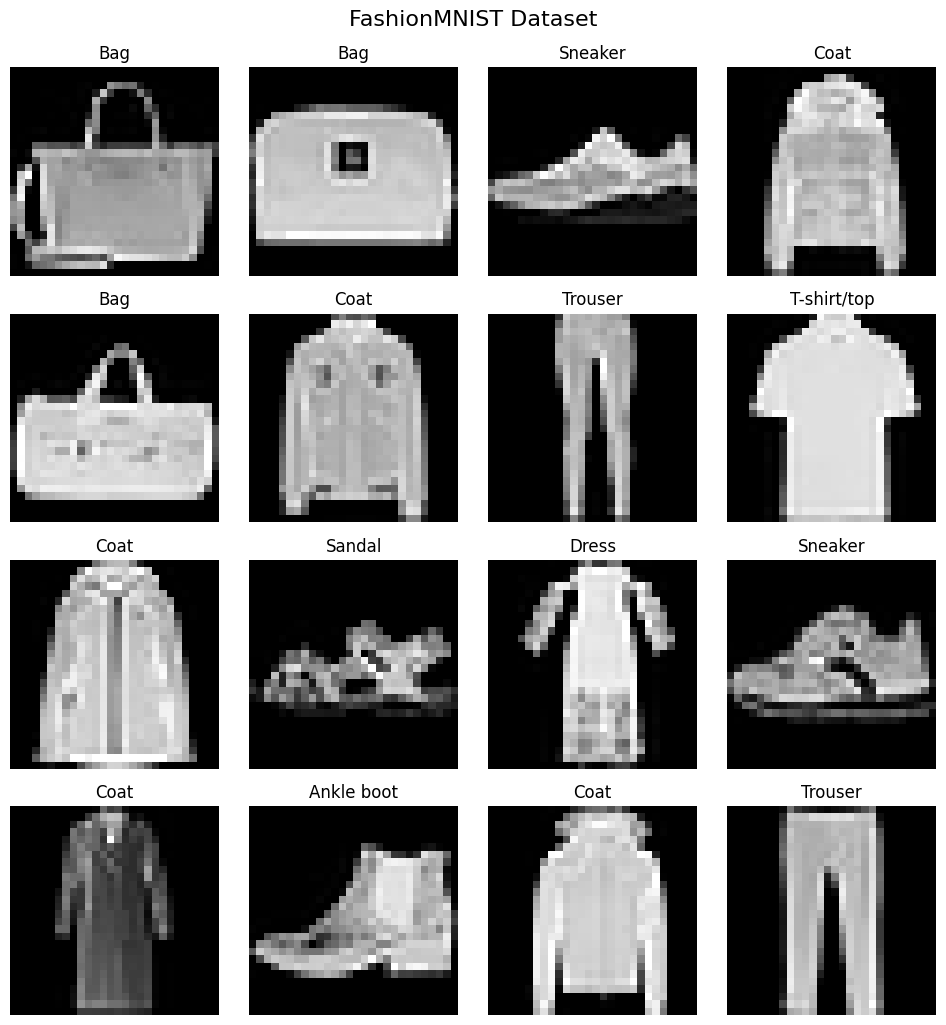
\includegraphics[scale=0.45]{figs/fmn data raw}
	 	\caption{بخشی از دیتاست
	 		\fm
	 	}
	 	\label{fig: fmn data}
	 \end{figure}
	 \begin{table}[H]
	 	\centering			
	 	\begin{tabular}{|c|c|}
	 		\hline
	 		تعداد کل تصاویر & ۷۰,۰۰۰ \\
	 		\hline
	 		مجموعه آموزش & ۶۰,۰۰۰ \\
	 		\hline
	 		مجموعه آزمون & ۱۰,۰۰۰ \\
	 		\hline
	 		ابعاد تصاویر & ۲۸×۲۸ پیکسل \\
	 		\hline
	 		نوع تصاویر & سیاه و سفید (تک‌کاناله) \\
	 		\hline
	 		محدوده مقادیر پیکسل‌ها & ۰ تا ۲۵۵ \\
	 		\hline
	 	\end{tabular}
	 	\caption{ویژگی‌های دیتاست 
	 		\lr{Fashion MNIST}
	 	}
	 	\label{tbl: fMNIST Chars}
	 \end{table}
	این مجموعه داده دارای ۱۰ کلاس مختلف است:
	\begin{itemize}
		\item تی‌شرت/تاپ
		\item شلوار
		\item پولیور
		\item پیراهن
		\item کت
		\item صندل
		\item پیراهن
		\item کفش ورزشی
		\item کیف
		\item چکمه
	\end{itemize}	
	\section{اضافه کردن نویز گاوسی
		\footnote{\lr{Gaussian Noise}}
		 به دیتاست}
	نویز گاوسی نوعی نویز می‌باشد که به تصویر اضافه می‌شود. 
	ضابطه زیر، تابع چگالی احتمال این نویز در دو بعد می‌باشد که برای تصاویر به کار برده می شود.
		\[ n(x,y) = \frac{1}{2\pi\sigma^2} e^{-\frac{(x-\mu_x)^2 + (y-\mu_y)^2}{2\sigma^2}} \]
		\begin{flushright}
			\begin{tabular}{r r}
				$\mu$ & میانگین\\
				$\sigma$ & انحراف معیار که پراکندگی نویز را نشان میدهد\\
				$\sigma^2$ & واریانس\\
			\end{tabular}
		\end{flushright}
		\newpage % optional
		\noindent
		در پردازش تصویر، فرمول اضافه کردن نویز گاوسی به تصویر به این صورت است:
		$$
		g(x,y) = f(x,y) + n(x,y)
		$$
		\begin{flushright}
			\begin{tabular}{r r}
				$g(x,y)$ & تصویر نویزی شده\\
				$f(x,y)$ & تصویر اصلی\\
				$n(x,y)$ & نویز گوسی که از توزیع نرمال با میانگین و انحراف معیار مشخص پیروی می‌کند\\
			\end{tabular}
		\end{flushright}
		در ابتدا به دیتاست
		\fm
		~ نویز گاوسی با واریانس 1.0 و میانگین 0 اضافه می‌کنیم. 
		از این داده‌ها به عنوان داده نویزی در طول تمرین استفاده خواهد شد.
		\footnote{در اصل هر تصویر به برداری به طول 784 تبدیل شده و در این تمرین مورد استفاده قرار می‌گیرد.}
		(بخشی از دیتاست در شکل 
		\ref{fig: fmn data noisy}
		)
	\begin{figure}[H]
		\centering
		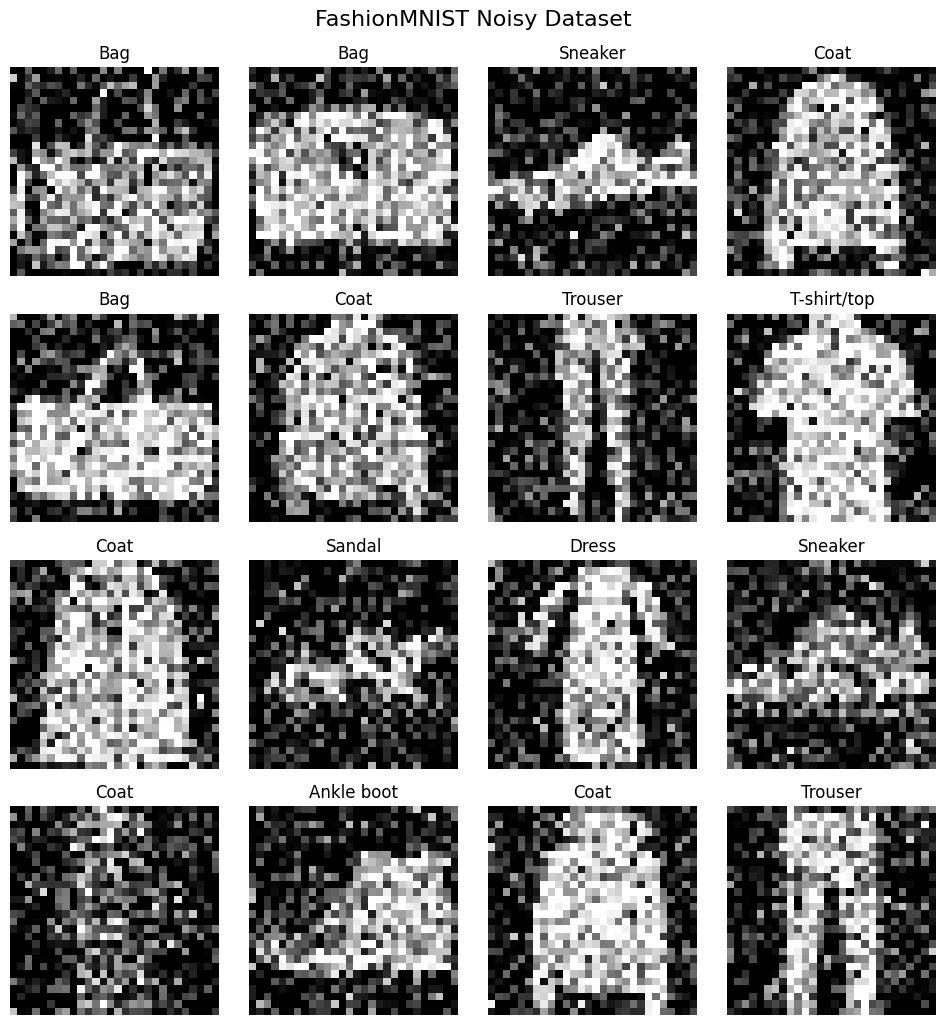
\includegraphics[scale=0.5]{figs/fmn data noisy}
		\caption{بخشی از دیتاست نویزی
			\fm
		}
		\label{fig: fmn data noisy}
	\end{figure}
	\newpage
	\section{کاهش نویز با 
		\pca
	}\label{sec: pca}
	\pca
	~ به عنوان یک روش کاهش بعد خطی، می‌تواند با بدست آوردن مولفه‌های مهم، اطلاعات مهم داده‌ها را حفظ کند. با در نظر گرفتن نویز وارد شده به تصویر به عنوان بخش غیر مهمی از اطلاعات موجود در داده‌ها، انتظار می رود \pca ~ بتواند کاهش نویز روی تصویر انجام دهد.
	مراحل کار بدین صورت است که ابتدا ماتریس $Q$
	\footnote{ماتریس 
		$Q$
		 شامل بردار های یکه و متعامد به یکدیگر می‌باشد. و بدین علت
		 $Q^{-1} = Q^T$
	}
	 که شامل بردارهای
	\lr{eigen}
	می باشد را برای ماتریس کواریانس 
	$\Sigma$
	بدست می ‌آوریم:
	$$
	\Sigma = Q\Lambda Q^{-1}
	$$
	$$
	Q = [q_1 \; q_2 \; \cdots \; q_d]
	$$
	$$
	\lambda_1 \geq \lambda_2 \geq \cdots \geq \lambda_d
	$$
	 سپس داده‌ها را بر روی مولفه‌های اصلی تصویر می‌کنیم:
	 $$
	 Y = (X - \mu)Q
	 $$
	 در نهایت داده‌ها را به بعد اصلی‌شان بر می‌گردانیم:
	 $$
	 X' = YQ^T‌+ \mu
	 $$
	 انتظار می رود با انتخاب مقدار مناسبی به عنوان تعداد مولفه‌های اصلی در نظر گرفته شده، این کاهش بعد و سپس بازگردانی داده‌ها به تعداد بعد اولیه باعث حذف مقدار زیادی نویز از تصویر بشود.\\
	 در تکلیف ارائه شده، مقدار 80 مولفه اصلی بهترین مقدار از بین 784 مقدار ممکن برای تعداد مولفه‌های اصلی بوده است. این مقدار به ما خطای 0239.0 را می‌دهد که بهترین خطای بازسازی در بین دیگر مقادیر مولفه‌های اصلی می باشد.(شکل 
	 \ref{fig: pca best k}
	 )
	 \begin{figure}[H]
	 	\centering
	 	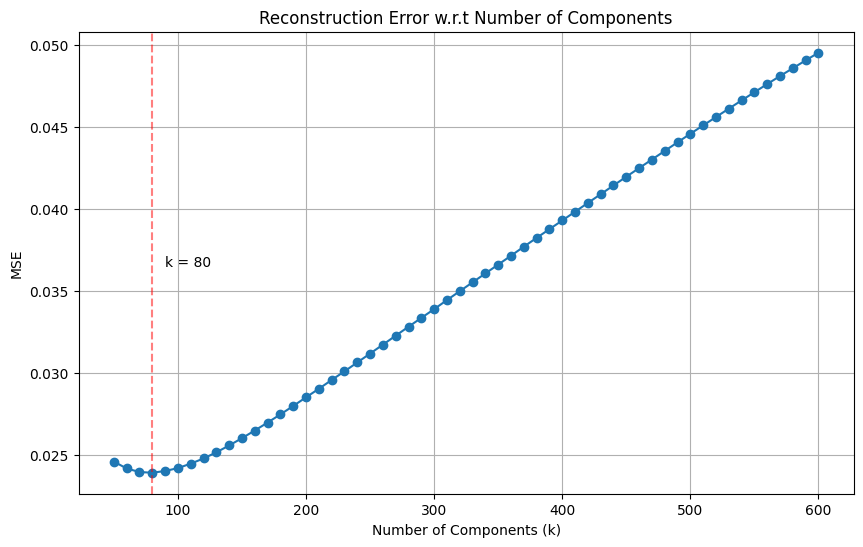
\includegraphics[scale=0.6]{figs/best k pca}
	 	\caption{پیدا کردن بهترین مقدار کاهش بعد با توجه به خطای بازسازی
	 	}
	 	\label{fig: pca best k}
	 \end{figure}
	\section{کاهش نویز با 
		\ae
	}\label{sec: ae}
	یک \ae، یک نوع شبکه عصبی می‌باشد که از دو بخش 
	\lr{Encoder}
	و 
	\lr{Decoder}
	تشکیل شده است. این نوع شبکه‌های عصبی می‌توانند به نوعی کاهش بعد خطی (در صورت داشتن تابع فعال ساز خطی) و یا غیر خطی (در صورت داشتن تابع فعال ساز غیر خطی) انجام دهند.\\
	یکی از استفاده‌هایی که از این نوع معماری شبکه می توان انجام داده این است که در ورودی به آن تصویر نویزی داده شود و برچسب هر تصویر نویزی، تصویر بدون نویز باشد. بدین ترتیب \ae ~ آموزش می‌بیند تا نگاشتی از تصویر نویزی به تصویر بدون نویز برقرار کند. که این همان مدلی می‌باشد که ما به آن نیاز داریم.\\
	شبکه‌ای با فریم ورک پایتورچ  متشکل از چند لایه
	\lr{Dense}
	و تابع فعال ساز
	\lr{ReLU}
	پیاده سازی شد. تعداد نورون‌های هر لایه به صورت زیر است:
	\[\text{\lr{Encoder}}:  784 \rightarrow 512 \rightarrow 256 \rightarrow 128 \]
	\[\text{\lr{Decoder}}:  128 \rightarrow 256 \rightarrow 512 \rightarrow 784 \]
	در شکل 
	\ref{fig: ae train test error}
	رفتار خطای آموزش و تست دیده می‌شود که دال بر یادگیری مناسب بدون بیش برازش
	\footnote{\lr{Overfit}}
	 می‌باشد. با این روش و هایپر پارامترهای گفته شده در جدول
	 \ref{tbl: ae hyparam}
	 به خطای 013.0 رسیده شد.
	 \begin{figure}[H]
	 	\centering
	 	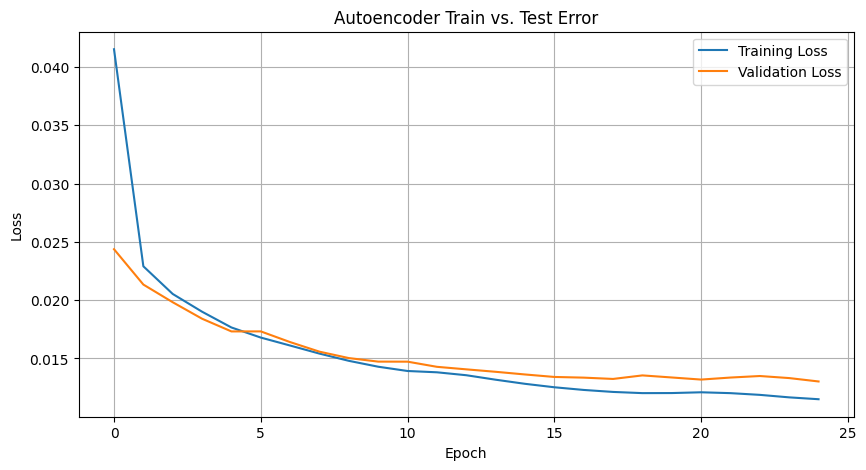
\includegraphics[scale=0.6]{figs/train test error ae}
	 	\caption{رویه خطای آموزش و تست \ae}
	 	\label{fig: ae train test error}
	 \end{figure}
	 \begin{table}[H]
	 	\centering
	 	\begin{tabular}{|c|c|}
	 		\hline
	 		نرخ یادگیری & 001.0\\
	 		\hline
	 		سایز هر دسته & 128	\\
	 		\hline
	 		\lr{Epochs} & 25\\
	 		\hline
	 	\end{tabular}
	 	\caption{هایپر پارامتر‌های  \lr{Autoencoder}}
	 	\label{tbl: ae hyparam}
	 \end{table}
	\section{نتایج}\label{sec: results}
	با مقایسه خطای گزارش شده در بخش‌های
	\ref{sec: ae}
	و
	\ref{sec: pca}
	انتظار می‌رود کاهش نویز با \ae ~ به نسبت \pca ~ بیشتر باشد. در شکل 
	\ref{fig: method comparison}
	می‌توان مقایسه ای بین تصویر نویزی، تصویر اصلی، کاهش نویز توسط \pca ~ و کاهش نویز توسط \ae ~ را مشاهده کرد.
	\begin{figure}[H]
		\centering
		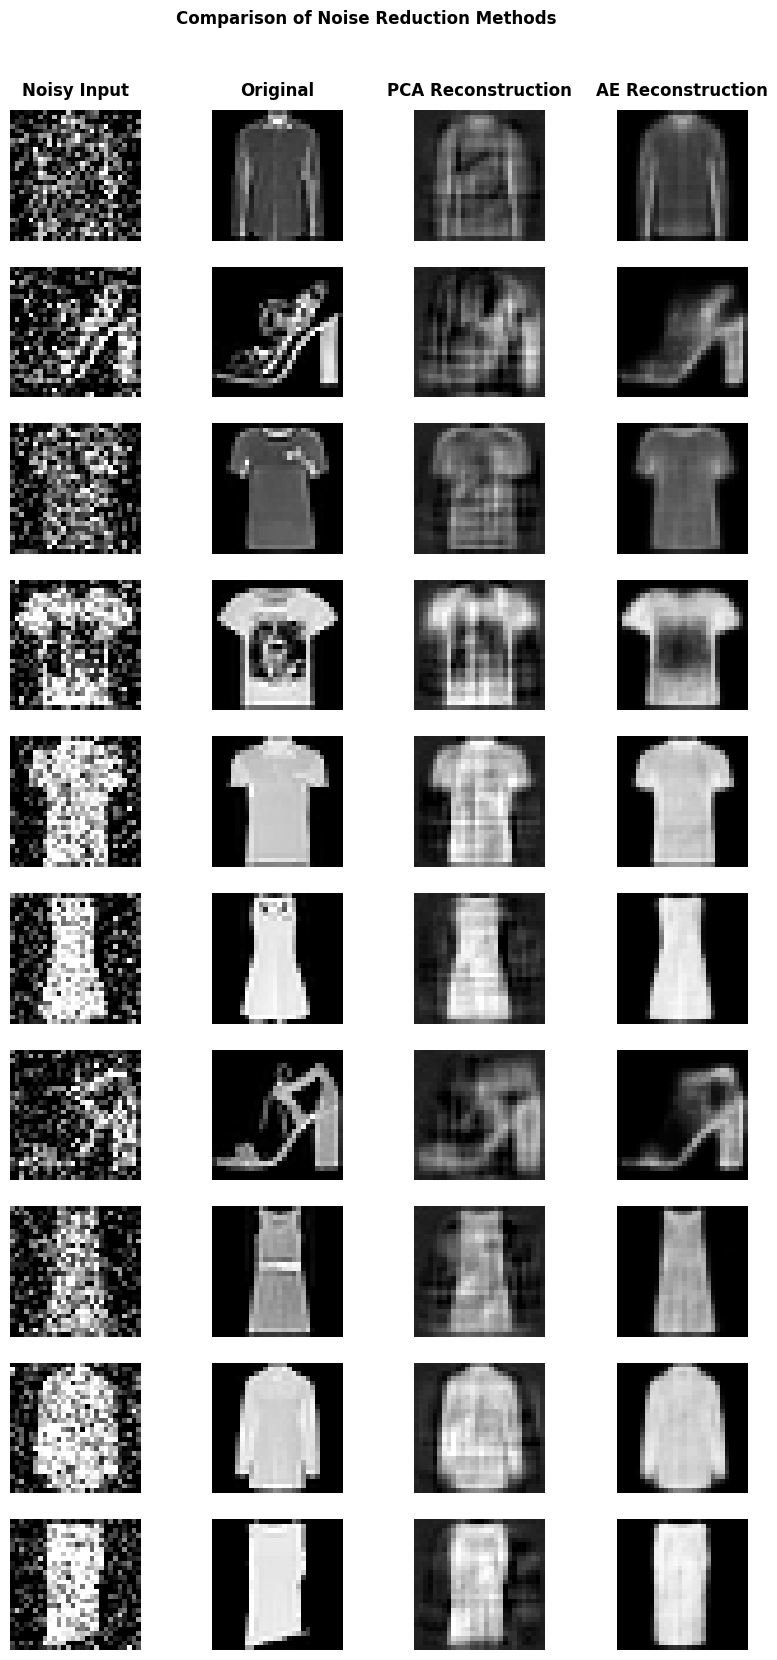
\includegraphics[scale=0.45]{figs/resutl comparison}
		\caption{رویه خطای آموزش و تست \ae}
		\label{fig: method comparison}
	\end{figure}
	\section{چالش‌: مقایسه عادلانه!}
	بزرگترین چالشی که در پیاده سازی تکلیف به آن برخورده شد، این بود که دیتاست بایستی از یک منبع دانلود شده و سپس با یکبار اضافه کردن نویز،‌ در کل تمرین و توسط هر روش استفاده و خطای روی آن گزارش می‌شد. این بدین علت بود که کتابخانه 
	\textit{\lr{Scikit Learn}}
برای متد \pca ~ و برای آموزش \ae ~ از کتابخانه
\textit{\lr{PyTorch}}
استفاده شده است. و اگر هر بار نویز گاوسی به هر یک از دیتاست ها برای هر متد اضافه می‌شود، تضمینی بر یکسانی نویز اضافه شده به تصویر نبود و همچنین لود کردن دیتاست از روی هر کتابخانه برای هر متد منجر به افزونگی نیز می‌گردید. برای همین، تنها یکبار دیتاست دانلود شد و در همان ابتدا نویز به آن اضافه شد و در کل تمرین مورد استفاده قرار گرفت تا در انتها مقایسه عادلانه تضمین گردد.
	
	\section{نتیجه‌گیری}
	با توجه به نتابج بدست آمده در بخش 
	\ref{sec: results}
	می‌توان به این نتیجه رسید که هر دو متد برای کاهش نویز کارساز بوده اند، اما متد \ae ~ بهتر از \pca ~ توانسته کاهش نویز را انجام دهد. که بنظر می‌رسد غیر خطی بودن کاهش بعد \ae ~ این قدرت را به مدل می‌دهد که روابط غیرخطی مهم را نیز در نظر بگیرد و تنها به روابط خطی (به مانند \pca) بسنده نکند.
\end{document}